\par The Muon Spectrometer~\cite{MUON-2010-01} is a composite detector designed to track  
muons with high precision and measure their \pT. These two goals are achieved by a set of 
sub-detectors encapsulated in a toroidal magnetic field supplied by superconducting 
toroids. Figure~\ref{fig:magnets} shows the toroidal arrangement of the superconducting coils.
Each coil is $5\times 26$~\SI{}{\m^2} in area, providing a magnetic field strength  
ranging from 0.5 to 2 T. 

\begin{figure}[!h]
	\centering
   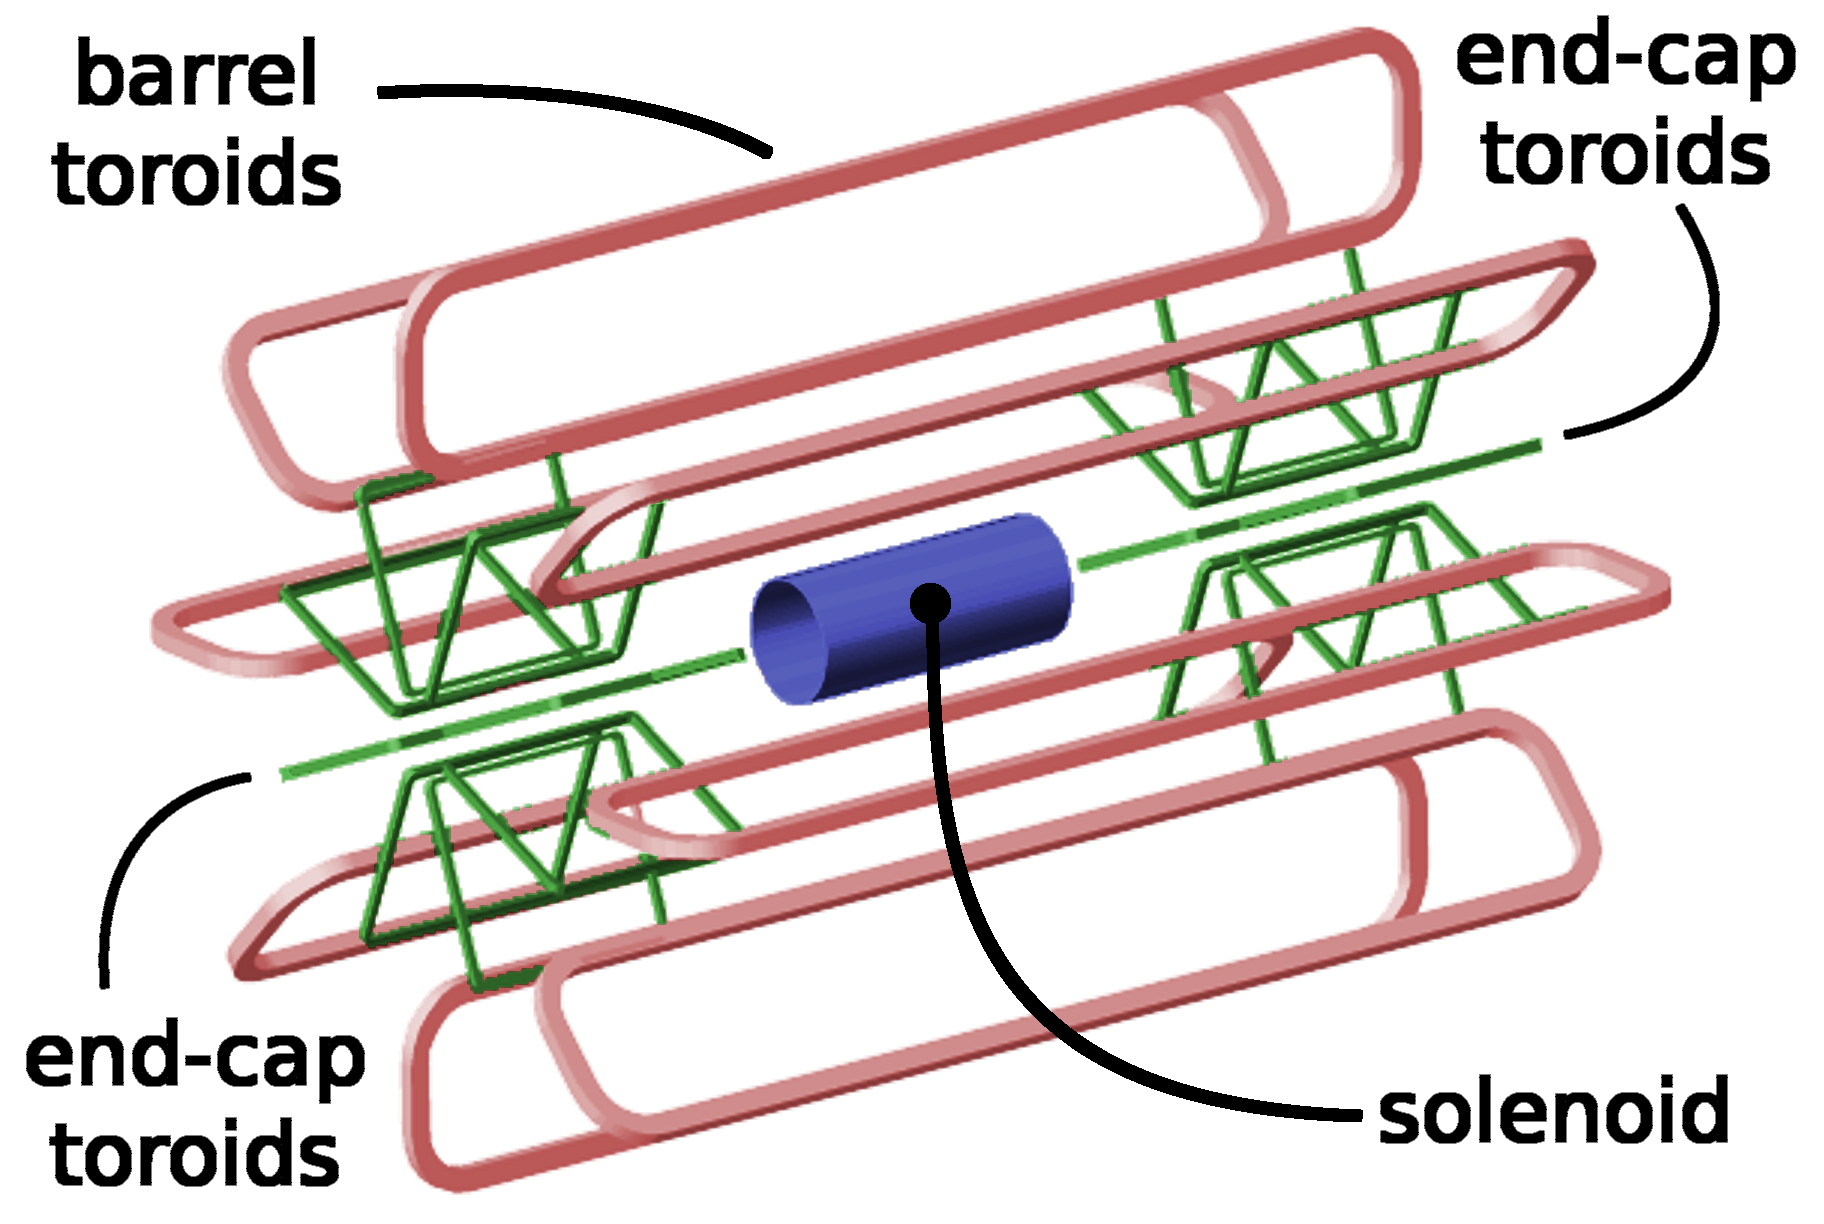
\includegraphics[width=0.8\textwidth]{figures/magnetSystems.png}
	\caption{The ATLAS magnetic system. The red toroid encapsulate the muon spectrometer sub-detectors, 
while the solenoid encapsulates the inner detector, which was discussed in Section~\ref{sec:ID}}
	\label{fig:magnets}
\end{figure}

\par All the sub-detectors in the muon spectrometer rely on ionizable gases. Their construction could be classified into 
drift chambers, multiwire proportional chambers (MWPCs) and resistive plate chambers (RPCs). In general the construction of each 
chamber is such that ionizable gas is enclosed in gas-tight structure made of a cathode and an 
anode, the arrangement of which supplies a near-constant electric field to the gas. As the muon  
ionizes the gas, the resultant electrons drift towards the anode and the positive ions towards 
the cathode, albeit at a much slower rate. The electrons create an avalanche near the anode. This avalanche in turn 
creates a pulse of current that is recorded as signal. On average the pulse width of the signal corresponds 
to the electron drift time. Because the electric field is near-constant, the drift velocity is well known. 
The pulse width and the electric field are therefore used to precisely locate the original position 
of the muon in the chamber. In a drift chamber (or drift tube) the cathode is the cylindrical  
casing and the anode is a thin wire at the center. As for the multiwire chamber the cathodes are parallel
planar walls while the anodes are multiple thin wires at the center of the cathode structure. 
The multiple wire arrangement enables the MWPC to handle higher muon rates than the 
drift tube. In a resistive plate chamber parallel planar plates of high resistivity act as the cathode 
and anode, with gas in the middle. Electric charges collected in the anode causes the electric field in the 
gas to momentarily drop, temporarily disabling the chamber; high resistivity minimizes the charge dissipation 
time, and consequently optimizes the chamber resolution. To put this into perspective, a \SI{e12}{\ohm\cm} anode 
has a \SI{10}{\m\s} charge dissipation time. 

\par Just like the arrangement of sub-detectors in the calorimeter, here a distinction is placed between 
barrel and end-cap sub-detectors. The strengths in each of them is always a trade-off between the measurement 
speed, spatial resolution and the ability to operate at high noise rates. Since there is more noise at high 
pseudorapidity, MWPCs are generally placed in the endcaps while drift tubes are placed in the barrel. A further
distinction is placed between precision sub-detectors and fast-measurement detectors, which are used 
for triggering for events that include a muon. 

\par RPCs are placed in the barrel component of the muon spectrometer specifically 
for triggering events with muons~\cite{1742-6596-280-1-012001}. The resistive plates are \SI{2}{\mm} thick and are made of bakelite, 
whose resistivity ranges between \SI{e9}{\ohm\cm} and~\SI{e12}{\ohm\cm}. The chambers have a \SI{2}{\mm} spacing that is enabled 
by insulating spacers, and are filled with 94.7\% of \ch{C2H2F4} as the ionizable gas.
The resistive plates are coated on the outside by graphite, which is of significantly 
lower resistivity. This arrangement helps in distributing the high voltage on the bakelite plates. Readout 
strips are placed immediately outside the graphite coating.   

\par Thin Gap Chambers~\cite{NAGAI1996219} (TGC) are placed in the end-caps for triggering events with muons of 
relatively lower \pT. A TGC is a multiwire chamber with graphite plates and \SI{50}{\micron} gold-plated 
tungsten wires with a \SI{1.8}{\mm} spacing. A mixture of 45\% n-Pentane and 55\% \ch{CO2} is filled in an air-tight 
\SI{2.8}{\mm} thick space between the graphite plates. This arrangement gives signal rise times below \SI{5}{\nano\s}, which 
is a very convenient time-frame for triggering events at the LHC.  

\par Monitored Drift Tube~\cite{DIEHL2012543} (MDT) chambers are used for 
precision measurements in the barrel and end-cap region. Each tube 
length ranges from \SI{0.9}{\m} to \SI{6.2}{\m}, with a constant diameter of \SI{3}{\cm}. 
The casing is a \SI{400}{\micron} thick aluminum 
alloy and the anode wire is a \SI{50}{\micron} \ch{W}-\ch{Re} wire, while the gas is a mixture of 93\% \ch{Ar} and 3\% \ch{CO2}. 
Each tube offers a spatial resolution of about \SI{100}{\micron}. An MDT chamber has two multilayers of tubes. A 
multilayer is made up of 3 to 4 layers of tubes supported by a beam structure 
shown in Figure~\ref{fig:mdt}. The alignment of these tubes is constantly monitored 
by x-ray beams to make sure that the tubes are not sagged. 

\begin{figure}[!h]
	\centering
   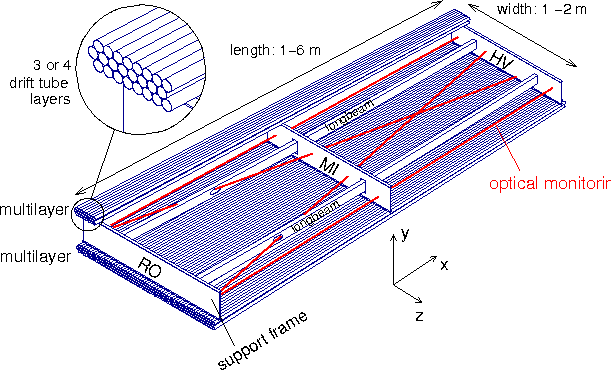
\includegraphics[width=0.8\textwidth]{figures/mdt_chamber.png}
	\caption{A cut-out of a Monitored Drift Tube chamber showing multi-layers of MDTs and the supporting beam structures}
	\label{fig:mdt}
\end{figure}

\par Cathode Strip Chambers~\cite{Argyropoulos:2009zz} (CSCs) are MWPCs that are placed in the end-caps for precision 
measurements because they have higher precision that MDTs and can handle the higher rates at high 
pseudorapidity. The plates are graphite and the wires are tungsten. The wire separation is \SI{2.54}{\mm} 
and the readout strips are \SI{5.08}{\mm} wide. The gas mixture used is 20\% \ch{Ar} and 20\% \ch{CO2}.
 The CSCs are segemented in 
$\phi$ on two wheels of eight chambers in the end-cap region, offering for layers of CSCs that a muon  
object has to traverse past. This arrangement give a \SI{60}{\micron} resolution on muon track position. 

\par Figure~\ref{fig:fullMu} shows the full muon spectrometer and all the sub-detectors. 

\begin{figure}
	\centering
   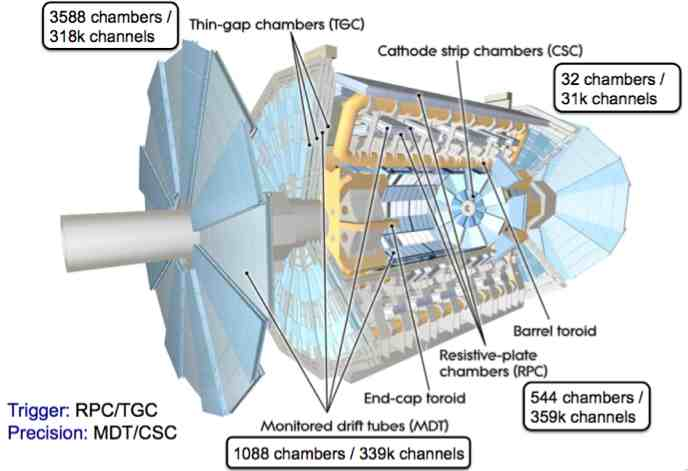
\includegraphics[width=0.8\textwidth]{figures/muSpecWhole.png}
	\caption{A cutaway view of the ATLAS Muon Spectrometer and its sub-detectors}
	\label{fig:fullMu}
\end{figure}
